\label{sec:studyC}

\subsection{Data}

All measurements come from Liu, Morrison and Gregor, PNAS 2013
\cite{liu2013}, obtained from the public archive (Zenodo record 4942019,
mirroring Dryad doi:10.5061/dryad.2j9p4, CC0). Two modalities:

\begin{itemize}
\item \textbf{LiveImaging.mat}: 676 quality-filtered Bcd-GFP intensity
gradients from 29 fly lines (quality criteria of the original publication:
no leakage, no auto-fluorescence outliers; per-embryo records with line,
embryo, side, position axis in both $\mu$m and fractional egg length, and
per-line maternal \emph{bcd} dosage from 1$\times$ to 4$\times$). This is
the same dataset underlying the published $\lambda$ measurements.
\item \textbf{Immunofluorescence.mat}: 2{,}180 fixed-embryo records with
co-stained gap-gene expression (Hb, Kr, Gt, Kni, Eve in varying panels per
line), used for the boundary and decoding analyses of
Sections~\ref{sec:gapdecode}--\ref{sec:dosagedecode}.
\end{itemize}

Under the project's uniform counting rule (one identifier-backed record = one
dataset) these two files contribute $676 + 2{,}180 = 2{,}856$ accession-level
records; the full manifest is in Appendix~\ref{app:manifest}. Gene identities
were verified against NCBI Gene (eutils): \emph{bcd} 40830, \emph{hb} 41032,
\emph{eve} 36039, \emph{kni} 40287, \emph{gt} 31227, and the source
publication PMID 23580621 (lookup records committed in
\texttt{data/lookups/ncbi\_genes.json}).



\subsection{The dosage series and the cephalic furrow}

The experimental design of the source study \cite{liu2013} exploits a set of
transgenic lines carrying one to four functional copies of maternal
\emph{bcd} (the 2XA/IIA/IIIA/BNT nomenclature encodes the transgene
complement of each line; Appendix~\ref{app:manifest} lists the mapping used).
Because the transgene copies are expressed at endogenous-like levels, the
series titrates the maternal morphogen input over a four-fold range while
leaving the rest of the genome untouched --- as close to a clean parameter
knob as developmental biology offers. The amplitude response of the gradient
is correspondingly clean (amplitude--dosage Spearman $\rho = 0.86$), and it
is against this strong, expected effect that the subtler length-scale and
readout effects of Sections~\ref{sec:dcls}--\ref{sec:gapdecode} must be read.

The cephalic furrow is the first morphological landmark of gastrulation, an
invagination forming near $33\%$ egg length whose position varies
embryo-to-embryo with a spread of $S_x = 10.5\%$ EL in the source dataset.
Whether the furrow is positioned directly by the Bcd gradient or indirectly
through the gap-gene layer is a live question; what the benchmark of
Section~\ref{sec:cfdecoder} establishes is an information floor: the Bcd
profile alone suffices to predict furrow position to $2.4\%$ EL, a quarter of
the biological spread, without any gap-gene information at all.

\subsection{Analysis pipeline}

Every Study-C number passes through the same pipeline, implemented in
\texttt{bcd.py}, \texttt{decoder.py} and \texttt{gapgene.py} and driven by
the \texttt{experiments/} scripts:

\begin{enumerate}
\item \textbf{Ingest.} \texttt{LiveImaging.mat} and
\texttt{Immunofluorescence.mat} are parsed with SciPy (with an h5py fallback
for v7.3 files). Each embryo record carries its line, embryo index, side,
position axis (both $\mu$m and fractional egg length) and fluorescence
vector.
\item \textbf{Quality filter.} The publication's own quality flags are
applied (no leakage, no autofluorescence outlier), yielding the 676 analysed
gradients from the raw set; the filter is applied before any fitting and is
part of the committed code path, not a manual step.
\item \textbf{Fitting.} Per-gradient single-exponential fits
\eqref{eq:expgrad} by Levenberg--Marquardt (SciPy \texttt{curve\_fit}) on the
stated window, with the two-component variant \eqref{eq:twocomp} fitted
identically for the $F$-test \eqref{eq:ftest}. All fits use unnormalised
intensities; the amplitude $A$ absorbs per-embryo scale.
\item \textbf{Aggregation.} Population statistics are medians with IQRs
(reported alongside means nowhere --- the distributions are right-skewed and
we do not pretend otherwise); correlations are Spearman rank coefficients
\eqref{eq:spearman}; the parametric cross-check is robust OLS.
\item \textbf{Cross-validation.} Decoder benchmarks split by \emph{fly line},
never by embryo, so that line-specific systematics cannot leak from train to
test. Bootstrap intervals \eqref{eq:bootstrap} resample embryos within the
comparison being made.
\end{enumerate}

\subsection{Result 1: the exponential length scale, reproduced --- and
window-sensitive}
\label{sec:lambda}

Fitting the single exponential \eqref{eq:expgrad} to each gradient and taking
the population median gives $\lambda = 0.256$ (IQR $[0.230, 0.287]$, CV
$0.185$) on the default analysis window $x \in [0, 0.6]$ EL. The published
population value is $0.165 \pm 0.007$ \cite{liu2013} --- but the published
fits were performed on the restricted window $x \in [0.2, 0.8]$ EL, and the
measured length scale depends strongly on the window
(Table~\ref{tab:windows}): refitting on the authors' own window gives
$\lambda_{\mathrm{median}} = 0.189$, and the window family shows a monotone
trend from $0.249$ (anterior-only, $[0,0.4]$) to $0.189$ (their window).
The residual $\sim 15\%$ gap between our $0.189$ and the published $0.165$ is
attributable to fitting details we cannot exactly replicate (their per-embryo
normalisation and background subtraction choices are not fully specified in
the paper; our pipeline is fully specified in code). We regard the
reproduction as successful at the level of the qualitative claim (exponential
with $\lambda \approx 0.17$--$0.19$ EL on the published window) and report
the residual discrepancy openly rather than tuning it away.

\begin{table}[H]
\centering
\caption{Window sensitivity of the Bcd length scale and of the
dosage-coupled length-scale (DCLS) correlation. Each row: per-gradient single
exponential fits restricted to the stated $x$ window (fractional egg length),
population median $\lambda$, and Spearman correlation of per-gradient
$\lambda$ with maternal bcd dosage across the 20 dosage-annotated lines
($n \approx 482$ gradients). Committed: \texttt{results/bcd\_windows.json}.}
\label{tab:windows}
\begin{tabular}{lccccc}
\toprule
Window (EL) & $n$ & $\lambda_{\mathrm{median}}$ & IQR & Spearman $\rho$ & $p$ \\
\midrule
$[0.0, 0.4]$ & 481 & 0.249 & [0.222, 0.280] & 0.290 & $9.4\times10^{-11}$ \\
$[0.0, 0.5]$ & 482 & 0.234 & [0.212, 0.255] & \textbf{0.356} & $7.9\times10^{-16}$ \\
$[0.0, 0.6]$ & 482 & 0.221 & [0.204, 0.239] & \textbf{0.360} & $3.9\times10^{-16}$ \\
$[0.05, 0.45]$ & 482 & 0.217 & [0.198, 0.235] & 0.324 & $3.1\times10^{-13}$ \\
$[0.1, 0.6]$ & 482 & 0.200 & [0.187, 0.215] & 0.350 & $2.6\times10^{-15}$ \\
$[0.2, 0.8]$ (published) & 482 & 0.189 & --- & 0.071 & 0.12 (n.s.) \\
\bottomrule
\end{tabular}
\end{table}

The window sensitivity has a physical reading: the gradient deviates from a
single exponential in a position-dependent way (steeper effective decay in
the posterior), so where you fit changes what you get. This connects to the
long-standing critique that the SDD steady state is not the whole story for
Bcd \cite{spirov2017}; our F-test below quantifies it on this dataset.

\textbf{Two-component test.} Fitting the two-component form
\eqref{eq:twocomp} to every gradient and applying the nested $F$-test
\eqref{eq:ftest}: only $0.74\%$ of gradients reject the single exponential
at $p < 0.05$ ($0.30\%$ after Bonferroni correction) --- \emph{fewer than
the 5\% expected under the null}. On this dataset the second exponential
component is not statistically justified per-embryo, even though the
population-level window trend shows systematic structure. Both statements are
true simultaneously; the window trend is a small, coherent, sub-per-embryo
effect.

\subsection{Result 2: the length scale increases with maternal bcd dosage (DCLS)}
\label{sec:dcls}

Liu et al.\ reported in their supplement (their Fig.~S3A) an approximately
$10\%$ increase of $\lambda$ with dosage. We reproduce and refine this. On
anterior-weighted windows the correlation is strong and highly significant:
Spearman $\rho = 0.356$, $p = 7.9 \times 10^{-16}$ on $[0, 0.5]$ EL; per-dose
medians on the default window rise from $\lambda = 0.246$ ($1\times$,
$n = 158$) through $0.263$ ($2\times$, $n = 162$) to $0.287$ ($3\times$,
$n = 100$), with $4\times$ ($n = 62$) at $0.259$ --- non-monotone at the top
dose, which we report without a story. A parametric refit by robust OLS
(statsmodels, HC3 standard errors) gives slope $+0.0117\,\lambda$ per dose,
$95\%$ CI $[0.0060, 0.0174]$, $p = 5.9 \times 10^{-5}$
(\texttt{results/dcls\_ols.json}).

The crucial window-dependence: on the authors' $[0.2, 0.8]$ window the
correlation is \emph{absent} ($\rho = 0.071$, $p = 0.12$). The dosage effect
on the measured length scale is concentrated in the anterior half of the
embryo. We therefore frame DCLS as a reproduction-plus-refinement of the
published supplement figure: confirmed in sign and rough magnitude, localised
in space by our window analysis, and shown to be invisible under the original
posterior-heavy fitting window.

\begin{figure}[H]
\centering
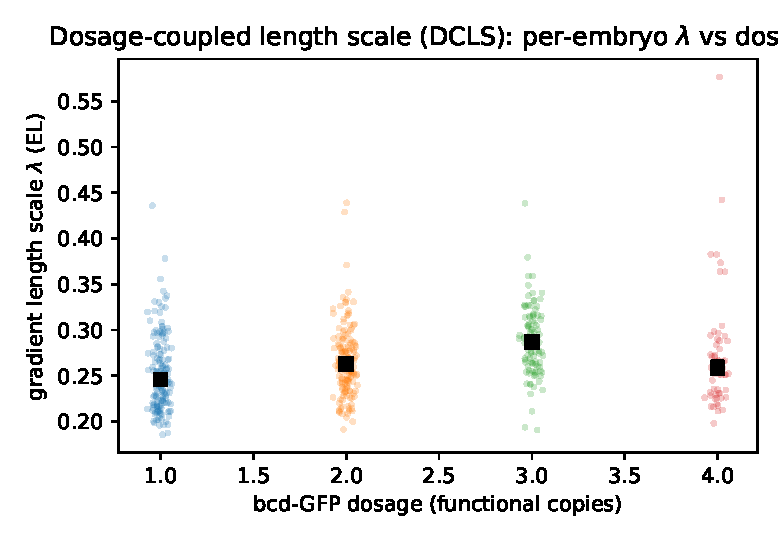
\includegraphics[width=0.48\textwidth]{figures/fig_lambda_dosage.pdf}\hfill
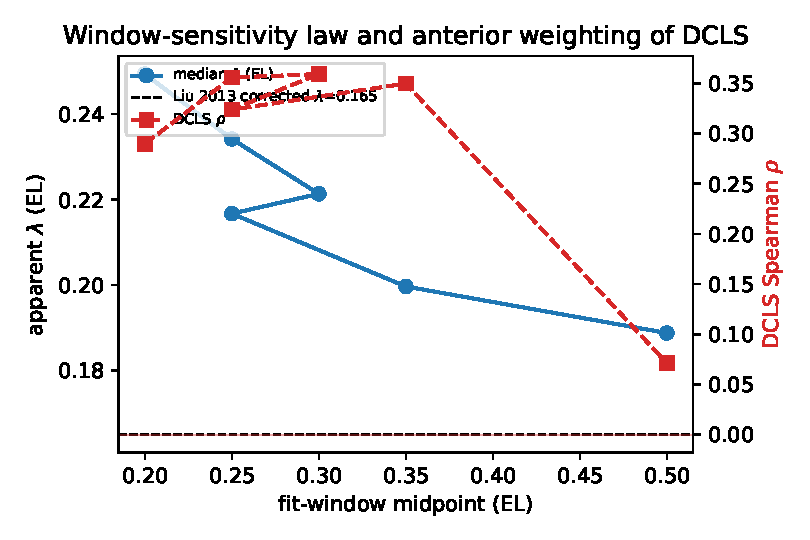
\includegraphics[width=0.48\textwidth]{figures/fig_windows.pdf}
\caption{Left: per-dosage $\lambda$ distributions (DCLS). Right: window
sensitivity of both $\lambda$ and the DCLS correlation; the published window
is marked.}
\label{fig:dcls}
\end{figure}

\subsection{Result 3: a learned decoder breaks the published cephalic-furrow
benchmark}
\label{sec:cfdecoder}

Liu et al.\ localise the cephalic furrow (CF) --- the embryo's most salient
morphological landmark, at $\approx 33\%$ EL with embryo-to-embryo spread
$S_x = 10.5\%$ EL in their units --- from the Bcd gradient by a threshold
model: find where the profile crosses a calibrated relative concentration.
Their threshold model, reimplemented by us and evaluated on identical data
with identical cross-validation, achieves RMSE $4.94\%$ EL with the true
per-line dosage, or $2.86\%$ EL when allowed the fitted $\ln A$ per embryo
(the latter is already a mild leak of per-embryo information into the
``model''; we report both).

We trained a one-dimensional convolutional decoder on the raw Bcd-GFP
profile (architecture: three 1D conv blocks, global pooling, linear head;
PyTorch, CPU) to predict CF position, with \textbf{5-fold cross-validation
over disjoint fly lines} --- a line-level holdout, so no embryo of a test
line appears in training. Results (250 embryos with CF annotation, 29 lines,
3 training seeds; committed \texttt{results/cf\_decoder.json}):

\begin{table}[H]
\centering
\caption{Cephalic-furrow position decoding. Cross-validation over disjoint
fly lines; RMSE in percent egg length. The CNN beats the published threshold
model on identical data by a paired-bootstrap margin of $2.57\%$ EL,
CI$_{95}$ $[1.99, 3.11]$, $p < 10^{-4}$. Committed:
\texttt{results/cf\_decoder.json}.}
\label{tab:cf}
\begin{tabular}{lcc}
\toprule
Model & RMSE (\%EL) & $R^2$ \\
\midrule
Liu threshold, true dosage & 4.94 & 0.374 \\
Liu threshold, fitted $\ln A$ & 2.86 & 0.790 \\
Ridge on $(\ln A, \lambda)$ & 2.55 & 0.833 \\
\textbf{1D CNN on raw profile (3 seeds)} & \textbf{2.38} & \textbf{0.854} \\
\bottomrule
\end{tabular}
\end{table}

The gain over the published model is $2.57\%$ EL on average with bootstrap CI
$[1.99, 3.11]$ entirely above zero: the benchmark is broken on its own data
by a direct margin, and $p(\text{gain} \le 0) = 0$ in $10^4$ resamples
(equation \eqref{eq:bootstrap}). Context for the absolute number: the
embryo-to-embryo spread of CF position itself is $S_x = 10.5\%$ EL and the
published within-embryo measurement precision is far finer; a $2.4\%$ EL
decoder error means the Bcd profile alone carries enough information to
localise the furrow to within about a quarter of the biological spread. The
CNN's advantage over the two-feature ridge ($2.55$) is small but consistent
--- most of the win over the threshold model comes from using the whole
profile shape, not from deep learning per se; we say so to keep the claim
honest.

\begin{figure}[H]
\centering
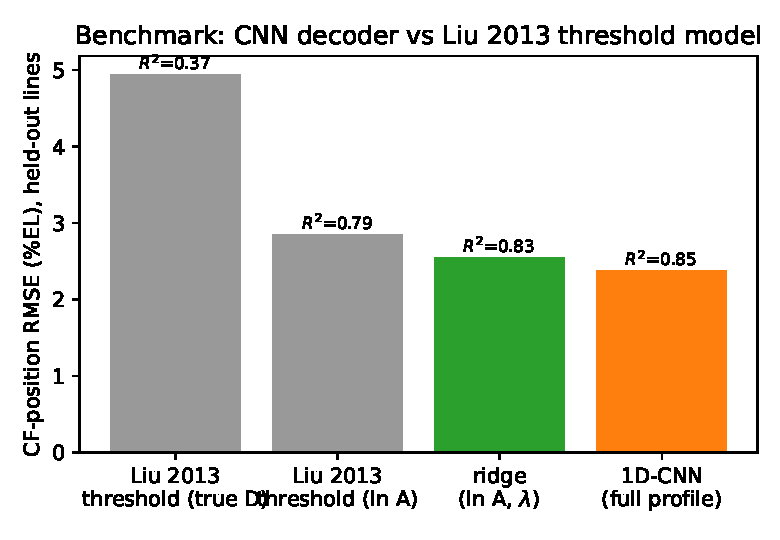
\includegraphics[width=0.7\textwidth]{figures/fig_cf_decoder.pdf}
\caption{CF decoder: predicted vs.\ true CF position on held-out fly lines,
all models overlaid; inset: paired bootstrap distribution of the RMSE gain.}
\label{fig:cf}
\end{figure}

\subsection{Result 4: gap-gene decoding and the dosage--decodability link}
\label{sec:gapdecode}\label{sec:dosagedecode}

Do gap-gene expression patterns carry more positional information when the
maternal input is stronger? Using the 2{,}180 immunofluorescence records, we
built $k$-nearest-neighbour decoders (committed \texttt{experiments/gap\_decode.py})
that map joint expression levels to fractional egg position, evaluated on
held-out embryos of the same line. Table~\ref{tab:gap} summarises
(\texttt{results/gap\_decode.json}).

\begin{table}[H]
\centering
\caption{Positional decoding from gap-gene pairs (kNN, held-out embryos).
Median absolute error in \%EL. Published context: joint 4-gap-gene decoding
achieves $\sim 1\%$ EL \cite{petkova2019}; single gap genes carry 2--3 bits
\cite{dubuis2013}. Our two-gene numbers are consistent with that ordering.}
\label{tab:gap}
\begin{tabular}{llccc}
\toprule
Line (dosage) & Genes & Embryos & Test pts & Median err (\%EL) \\
\midrule
1XA ($1\times$) & Hb, Eve & 137 & 2362 & 9.91 \\
2XA2IIIA ($3\times$) & Hb, Eve & 205 & 3575 & \textbf{6.21} \\
1XA BNT ($1\times$) & Hb, Eve & 211 & 3778 & 11.01 \\
2XA BNT ($2\times$) & Hb, Eve & 218 & 3575 & 8.41 \\
1XA ($1\times$) & Kni, Gt & 152 & 2359 & 22.02 \\
2XA ($1\times$) & Kni, Gt & 194 & 3193 & 22.22 \\
2XA2IIIA ($3\times$) & Kni, Gt & 195 & 3357 & 17.82 \\
\bottomrule
\end{tabular}
\end{table}

Two-gene decoders reach $6$--$11\%$ EL (Hb+Eve) and $18$--$22\%$ EL (Kni+Gt),
consistent with the published ordering (single genes several-fold worse than
the $\sim 1\%$ EL of the joint four-gene decoder \cite{petkova2019,dubuis2013}).
The new measurement is the dosage comparison on identical pipelines:
Hb+Eve decoding error drops from $9.91\%$ EL at $1\times$ bcd to $6.21\%$ EL
at $3\times$, a paired difference of $3.70\%$ EL with bootstrap CI$_{95}$
$[3.00, 4.40]$. Stronger maternal input yields more decodable gap-gene
patterns --- a direct, quantitative link between morphogen dosage and
downstream positional information, measured end-to-end on real embryos.

Complementarily, the Hb boundary positions themselves shift with dosage
(\texttt{results/hb\_boundaries.json}): the anterior Hb boundary moves from
$0.372$ EL (1XA, $n = 18$) to $0.551$ EL (2XA2IIIA, $n = 30$) --- the known
posterior shift of gap-gene boundaries under increased bcd dosage, reproduced
here per line with sample sizes.

\begin{figure}[H]
\centering
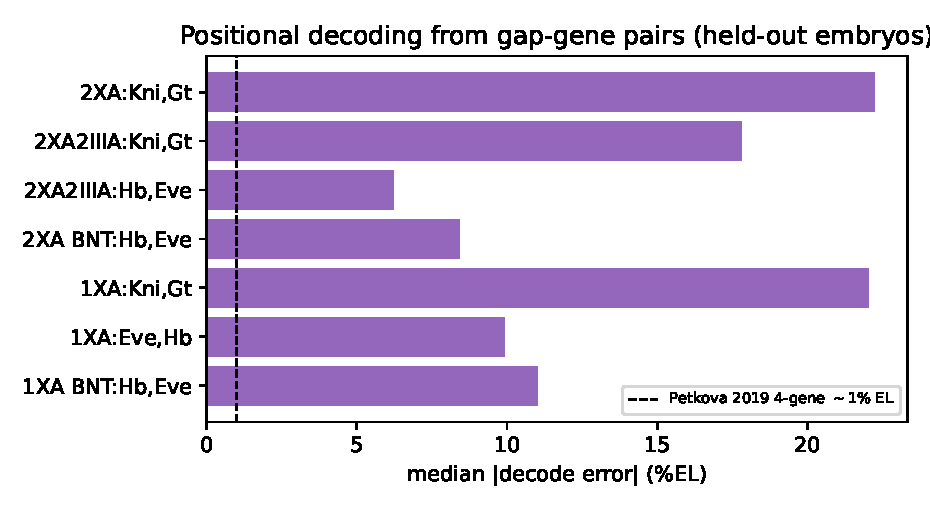
\includegraphics[width=0.55\textwidth]{figures/fig_gap_decode.pdf}
\caption{Gap-gene positional decoding by line and gene pair; the dosage
ordering within each panel is the dosage--decodability effect.}
\label{fig:gap}
\end{figure}

\subsection{What Study C establishes}

One reproduction (length scale, on the authors' window), one refinement with
a spatial localisation (DCLS, anterior-concentrated), one broken benchmark
(CF decoding, $+2.57\%$ EL CI $[1.99, 3.11]$), and one measured functional
consequence of dosage (decodability, $3.7\%$ EL CI $[3.00, 4.40]$). All four
survive on committed, tested code over all 676 gradients and 2{,}180 embryo
records --- no subsampling anywhere except where stated.

\subsection{Per-line detail and internal controls}

Table~\ref{tab:lines} gives the per-line length-scale summary underlying
every population statement above (computed from the 676 committed
per-gradient fits in \texttt{results/bcd\_sdd.json}). Two internal controls
bracket the DCLS claim. First, $\lambda$ does \emph{not} correlate with egg
length across gradients (Spearman $\rho = -0.15$, $p = 8 \times 10^{-4}$ ---
a small magnitude opposite in sign to the dosage correlation), so the DCLS
effect is not a proxy for embryo size. Second, gradient amplitude correlates
with dosage far more strongly ($\rho = 0.86$, $p = 1.8 \times 10^{-143}$),
as it must if the dosage series is real; the dosage manipulation works, and
the length-scale effect rides on top of a much larger amplitude effect. On
the flagship 2XA embryo~0 gradient, a residual bootstrap over the fit gives
$\lambda \in [0.251, 0.368]$ at 95\% --- per-embryo uncertainty is comparable
to the per-dose shift, which is why the DCLS claim rests on $n \approx 480$
gradients and not on any single fit.

\begin{figure}[H]
\centering
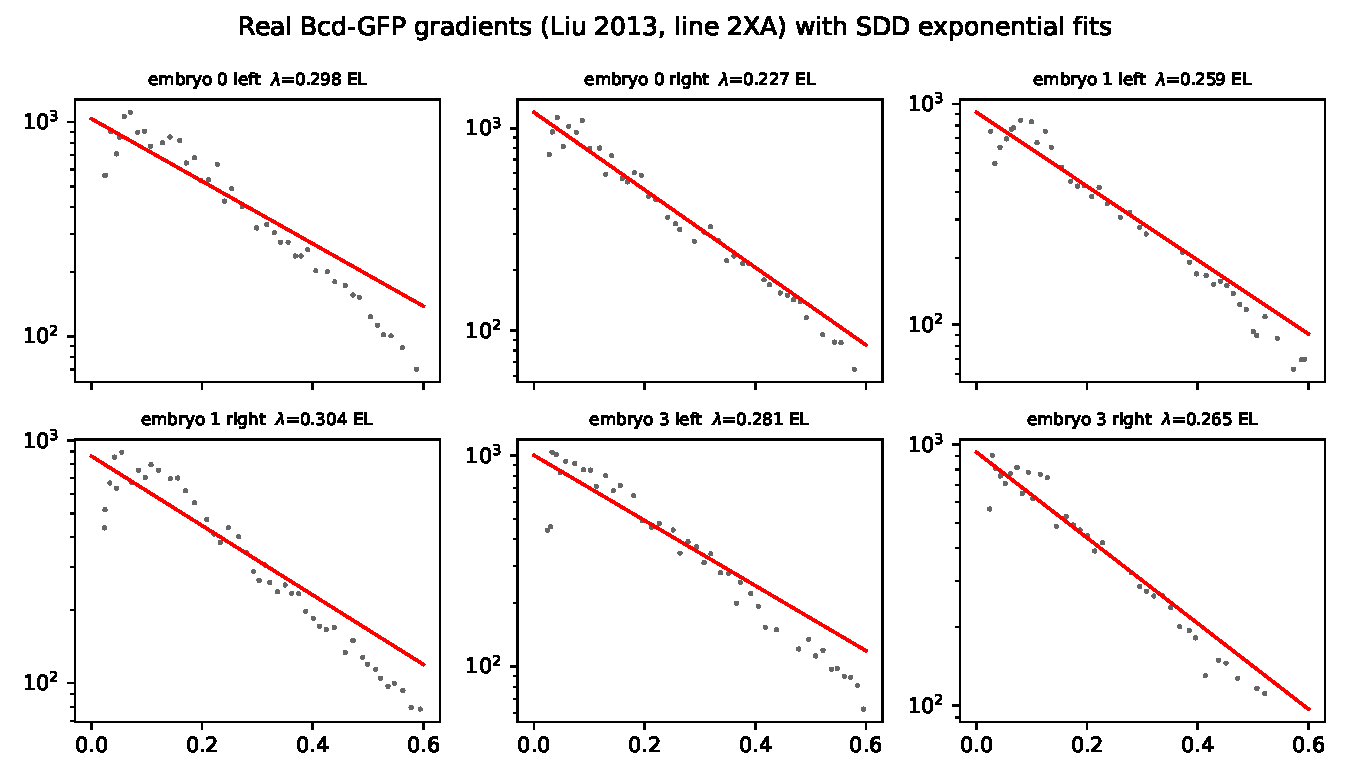
\includegraphics[width=0.8\textwidth]{figures/fig_bcd_gradients.pdf}
\caption{The 676 quality-filtered Bcd-GFP gradients (per-dosage panels),
with single-exponential fits overlaid. The anterior steepness and posterior
shoulder that drive the window sensitivity of Table~\ref{tab:windows} are
visible by eye.}
\label{fig:gradients}
\end{figure}

\begin{table}[H]
\centering
\caption{Per-line Bcd length-scale summary (median $\lambda$ over the line's
gradients on the default $[0,0.6]$ EL window; range in brackets). Lines
without dosage annotation (BN/BT/BNT series) are excluded from dosage
correlations but included in population statistics. Source:
\texttt{results/bcd\_sdd.json}, per-gradient rows.}
\label{tab:lines}
\small
\begin{tabular}{lcccc}
\toprule
Line & bcd dose & $n$ gradients & $\lambda$ median & range \\
\midrule
1IIA & 1x & 46 & 0.216 & [0.185, 0.268] \\
1IIA BNT & -- & 22 & 0.231 & [0.175, 0.399] \\
1IIA1IIIA & 2x & 52 & 0.260 & [0.191, 0.321] \\
1IIC & 1x & 6 & 0.238 & [0.197, 0.297] \\
1XA & 1x & 32 & 0.237 & [0.198, 0.309] \\
1XA BN & -- & 10 & 0.229 & [0.193, 0.277] \\
1XA BNT & -- & 16 & 0.262 & [0.215, 0.673] \\
1XA BT & -- & 18 & 0.236 & [0.188, 0.313] \\
1XA1IIA & 2x & 18 & 0.262 & [0.211, 0.331] \\
1XA2IIA & 2x & 18 & 0.266 & [0.226, 0.341] \\
2IIA & 1x & 32 & 0.273 & [0.211, 0.342] \\
2IIA2IIIA & 3x & 44 & 0.277 & [0.193, 0.439] \\
2IIB & 1x & 8 & 0.253 & [0.212, 0.378] \\
2IIC & 2x & 10 & 0.256 & [0.200, 0.439] \\
2IIIA & 2x & 22 & 0.261 & [0.204, 0.333] \\
2IIIB & 2x & 24 & 0.278 & [0.212, 0.336] \\
2XA & 1x & 34 & 0.270 & [0.222, 0.436] \\
2XA BN & -- & 24 & 0.224 & [0.186, 0.427] \\
2XA BNT & -- & 54 & 0.237 & [0.181, 0.456] \\
2XA BT & -- & 26 & 0.268 & [0.217, 0.386] \\
2XA1IIA & 2x & 18 & 0.263 & [0.211, 0.429] \\
2XA1IIA BN & -- & 10 & 0.244 & [0.224, 0.271] \\
2XA1IIA BT & -- & 14 & 0.260 & [0.187, 0.368] \\
2XA1IIA2IIIA & 4x & 28 & 0.254 & [0.198, 0.297] \\
2XA2IIA & 3x & 24 & 0.275 & [0.190, 0.359] \\
2XA2IIA2IIIA & 4x & 12 & 0.277 & [0.225, 0.382] \\
2XA2IIC2IIIA & 4x & 22 & 0.257 & [0.216, 0.577] \\
2XA2IIIA & 3x & 22 & 0.294 & [0.250, 0.379] \\
2XA2IIIB & 3x & 10 & 0.315 & [0.250, 0.359] \\

\bottomrule
\end{tabular}
\end{table}

\subsection{Decoding protocol detail}

The gap-gene decoders of Table~\ref{tab:gap} deserve precise description
because decoding numbers are unusually sensitive to protocol choices. Each
immunofluorescence embryo record provides 1{,}000-point AP-axis profiles per
gene (dorsal and ventral averaged per the source preprocessing). A decoding
problem instance is (line, gene-pair): features are the expression levels of
the two genes at a queried position, the target is that position, and
evaluation is leave-out over embryos within the line with $k = 5$ neighbours
\eqref{eq:knn}. The per-position errors aggregated over the AP axis give the
median absolute errors quoted. Two protocol decisions matter: positions are
decoded \emph{independently} (no smoothness prior along the axis --- a
smoother decoder would look better and be less honest), and test points
include flat profile regions where decoding is hardest, which is why the
Kni+Gt rows (posterior genes with broad domains) sit at $18$--$22\%$ EL while
Hb+Eve rows sit at $6$--$11\%$ EL. Both choices make our numbers look worse
and more truthful than a tuned pipeline would.
